% The Gwangyang earthquake sequence, 2012-2026: study plan.
% Every number in this file comes from facts.tex (macro \F with a fact key), which notebooks/90_study_plan_report.ipynb writes from facts.json;
% the appendix table (tab_decisions.tex) is written by the same notebook from docs/decisions.csv.
% Compile: tectonic -X compile report.tex
\documentclass[11pt,a4paper]{article}
\usepackage[a4paper,top=2.2cm,bottom=2.4cm,left=2.3cm,right=2.3cm,footskip=1.0cm]{geometry}
\usepackage{fontspec}
\usepackage{unicode-math}
\setmainfont{texgyretermes}[Extension=.otf,UprightFont=*-regular,BoldFont=*-bold,ItalicFont=*-italic,BoldItalicFont=*-bolditalic]
\setsansfont{texgyreheros}[Extension=.otf,UprightFont=*-regular,BoldFont=*-bold,ItalicFont=*-italic,BoldItalicFont=*-bolditalic]
\setmathfont{texgyretermes-math.otf}
\usepackage{microtype}
\usepackage{graphicx}
\usepackage{booktabs}
\usepackage{array}
\usepackage{tabularx}
\usepackage{longtable}
\usepackage{xcolor}
\usepackage[font=small,labelfont=bf,labelsep=period,skip=5pt,justification=justified]{caption}
\usepackage[authoryear,round]{natbib}
\usepackage[explicit]{titlesec}
\usepackage{enumitem}
\usepackage{placeins}
\usepackage[hidelinks,pdfusetitle]{hyperref}

\definecolor{headblue}{RGB}{28,57,120}
\titleformat{\section}{\sffamily\bfseries\large\color{headblue}}{\thesection}{0.6em}{#1}
\titleformat{\subsection}{\sffamily\bfseries\normalsize}{\thesubsection}{0.6em}{#1}
\titlespacing*{\section}{0pt}{12pt plus 3pt minus 2pt}{5pt plus 1pt}
\titlespacing*{\subsection}{0pt}{8pt plus 2pt minus 2pt}{3pt plus 1pt}
\setlength{\parskip}{0pt}
\setlength{\parindent}{1.2em}
\linespread{1.05}
\setlength{\bibsep}{2pt plus 1pt}
\renewcommand{\bibfont}{\small}
\setlist{itemsep=1pt,topsep=3pt,leftmargin=1.6em}
\renewcommand{\topfraction}{0.95}
\renewcommand{\bottomfraction}{0.8}
\renewcommand{\textfraction}{0.05}
\renewcommand{\floatpagefraction}{0.75}
\setcounter{topnumber}{2}
\setcounter{totalnumber}{3}

% facts.tex -- written by notebooks/90_study_plan_report.ipynb from facts.json; do not edit by hand.
% generated 2026-10-16T16:41:02+09:00; 141 macros.
\makeatletter
\newcommand\FactDef[2]{\expandafter\def\csname fact@#1\endcsname{#2}}
\DeclareRobustCommand\F[1]{\ifcsname fact@#1\endcsname\csname fact@#1\expandafter\endcsname\else\PackageError{facts}{Undefined fact #1}{Add it to notebook 90}\fi}
\makeatother
\FactDef{aud.all}{8}
\FactDef{aud.n26}{0}
\FactDef{aud.w0}{10}
\FactDef{aud.w1}{59}
\FactDef{aud.z0}{14}
\FactDef{aud.z1}{4}
\FactDef{cen.lat}{35.0000}
\FactDef{cen.lon}{127.7286}
\FactDef{chk.max}{0.30}
\FactDef{chk.med}{0.00}
\FactDef{chk.n}{950}
\FactDef{chk.p95}{0.10}
\FactDef{data.n100_2013}{11}
\FactDef{data.n100_2021}{61}
\FactDef{data.n100_max}{82}
\FactDef{data.sd_kigam}{3,543}
\FactDef{data.sd_mara}{237,867}
\FactDef{dec.n}{34}
\FactDef{dec.n_gd}{20}
\FactDef{dec.open}{G-D12, G-D19}
\FactDef{f4.n_nec}{18}
\FactDef{f4.n_none}{8}
\FactDef{f4.n_part}{4}
\FactDef{f4.nsta}{61}
\FactDef{f4.pct}{99.8}
\FactDef{g2.periods}{147}
\FactDef{g2.units}{110}
\FactDef{g2.valid}{144}
\FactDef{g2.windows}{22,078}
\FactDef{gwyb.e1}{2016-09-23}
\FactDef{gwyb.e2}{2017-07-26}
\FactDef{gwyb.e3}{2023-07-02}
\FactDef{gwyb.e4}{2026-10-06}
\FactDef{gwyb.n_ev}{1,404}
\FactDef{gwyb.n_new}{9}
\FactDef{gwyb.s1}{2013-01-10}
\FactDef{gwyb.s2}{2016-10-15}
\FactDef{gwyb.s3}{2017-08-11}
\FactDef{gwyb.s4}{2023-07-03}
\FactDef{gwyb.t1}{−125.5}
\FactDef{gwyb.t2}{+94.6}
\FactDef{gwyb.t3}{−95.2}
\FactDef{gwyb.t4}{+45.6}
\FactDef{kma.n10}{25}
\FactDef{kma.n10_other}{14}
\FactDef{kma.n10_other_years}{2014 (3), 2016 (1), 2017 (1), 2019 (2), 2020 (1), 2021 (1), 2023 (2), 2026 (3)}
\FactDef{kma.n10_seq}{11}
\FactDef{kma.n5}{14}
\FactDef{kma.n5_extra}{22 April 2019 (ML 1.0, 3.5 km); 26 June 2023 (ML 1.5, 3.5 km); 26 May 2026 (ML 1.6, 0.8 km)}
\FactDef{meta.date}{16 October 2026}
\FactDef{nec.files}{18}
\FactDef{nec.jobs}{11}
\FactDef{nec.rec}{8}
\FactDef{ori.n60}{39}
\FactDef{ori.n_changed60}{9}
\FactDef{ori.n_meas}{104}
\FactDef{ori.n_none}{6}
\FactDef{ori.none}{CHR, HAC, JAH, JAS, SAC, YES}
\FactDef{p.box_lat}{34.30–35.70° N}
\FactDef{p.box_lon}{126.93–128.53° E}
\FactDef{p.err}{5}
\FactDef{p.fmf_band}{5–20}
\FactDef{p.fmf_mad}{10}
\FactDef{p.fmf_minsta}{4}
\FactDef{p.fmf_pre}{1}
\FactDef{p.fmf_snr}{2}
\FactDef{p.fmf_win}{4}
\FactDef{p.fs}{100}
\FactDef{p.gap}{180}
\FactDef{p.ml_nsta}{3}
\FactDef{p.ml_snr}{2}
\FactDef{p.n_p}{3}
\FactDef{p.n_picks}{6}
\FactDef{p.n_s}{3}
\FactDef{p.num}{7}
\FactDef{p.obscc}{4}
\FactDef{p.pmin}{0.2}
\FactDef{p.radius}{5}
\FactDef{p.rms}{1}
\FactDef{p.xc_band}{5–20}
\FactDef{p.xc_cc}{0.7}
\FactDef{p.xc_interp}{1,000}
\FactDef{p.xc_win}{0.5}
\FactDef{port.n_edit}{12}
\FactDef{port.n_ident}{95}
\FactDef{prev.depth}{13.9}
\FactDef{prev.err}{3.2, 2.2 and 5.5}
\FactDef{prev.hext}{141}
\FactDef{prev.n}{11}
\FactDef{prev.nboot}{1,000}
\FactDef{prev.zext}{45}
\FactDef{seq.big_kst}{2021-08-28 07:03}
\FactDef{seq.big_utc}{2021-08-27 22:03:22}
\FactDef{seq.ml}{1.1–2.2}
\FactDef{seq.n}{11}
\FactDef{seq.n21}{6}
\FactDef{seq.n26}{5}
\FactDef{seq.t21}{20 July to 28 August 2021}
\FactDef{seq.t26}{1 January to 4 February 2026}
\FactDef{smoke.dP}{0.019}
\FactDef{smoke.dS}{0.020}
\FactDef{smoke.depth}{15.22}
\FactDef{smoke.dtmax}{1.23}
\FactDef{smoke.epi}{0.12}
\FactDef{smoke.kma}{7 of 7}
\FactDef{smoke.npk}{458}
\FactDef{smoke.sparse}{10}
\FactDef{sta.n}{110}
\FactDef{sta.n100_2013}{11}
\FactDef{sta.n100_2016}{39}
\FactDef{sta.n100_2021}{61}
\FactDef{sta.n100_2026}{82}
\FactDef{sta.n50_2013}{4}
\FactDef{sta.n50_2016}{11}
\FactDef{sta.n50_2021}{15}
\FactDef{sta.n50_2026}{19}
\FactDef{sta.n60_2013}{8}
\FactDef{sta.n60_2016}{16}
\FactDef{sta.n60_2021}{24}
\FactDef{sta.n60_2026}{29}
\FactDef{sta.n_EL}{14}
\FactDef{sta.n_HG}{82}
\FactDef{sta.n_HH}{14}
\FactDef{sta.n_kg}{8}
\FactDef{sta.n_ks}{102}
\FactDef{sta.n_temp}{5}
\FactDef{sta.nearest}{GWYB (7.1 km)}
\FactDef{sta.temp}{DAYAT, GEJAT, GWYBT, NAWBT, SUCAT}
\FactDef{stat.freeze}{d724acfddcd608dd}
\FactDef{stat.freeze_time}{2026-10-16 12:51}
\FactDef{stat.kigam_err}{0}
\FactDef{stat.kigam_files}{10,629}
\FactDef{stat.kigam_req}{3,543}
\FactDef{stat.links}{711,715}
\FactDef{stat.pull_done}{760}
\FactDef{stat.pull_tb}{6.9}
\FactDef{stat.pull_tot}{760}
\FactDef{stat.time}{2026-10-16 16:40 KST}
\FactDef{stat.verify_missing}{222}
\FactDef{win.end}{2026-10-06}
\FactDef{win.start}{2012-12-20}

% facts_pilot.tex -- written by notebooks/91_pilot_episode_events.ipynb; do not edit by hand.
\FactDef{pilot.days21}{1–64 and 184–245 (1 January to 5 March and 3 July to 2 September)}
\FactDef{pilot.days26}{1–51 and 140–190 (1 January to 20 February and 20 May to 9 July)}
\FactDef{pilot.dd_n}{31}
\FactDef{pilot.dd_std}{110 m east, 188 m north and 214 m in depth}
\FactDef{pilot.e1_kma}{0.29}
\FactDef{pilot.e1_new}{0.73}
\FactDef{pilot.fail}{No. 11 (2021-08-27 02:09) and No. 12 (2021-08-27 18:44)}
\FactDef{pilot.hyp_std}{749 m, 366 m and 1165 m}
\FactDef{pilot.kmao}{26 May 2026, 15:45 UTC, ML 1.6}
\FactDef{pilot.loo21}{0.37}
\FactDef{pilot.loo26}{0.20}
\FactDef{pilot.loo_rms}{0.30}
\FactDef{pilot.low21}{0.60}
\FactDef{pilot.ml_new}{−0.6 to 1.1}
\FactDef{pilot.ml_new_med}{0.3}
\FactDef{pilot.n}{33}
\FactDef{pilot.n_amp21}{6}
\FactDef{pilot.n_both}{19}
\FactDef{pilot.n_cc07}{15}
\FactDef{pilot.n_kmao}{1}
\FactDef{pilot.n_new}{21}
\FactDef{pilot.n_noise}{19}
\FactDef{pilot.n_poor}{9}
\FactDef{pilot.n_samesp}{20}
\FactDef{pilot.n_seq}{11}
\FactDef{pilot.noiseP}{0.46}
\FactDef{pilot.noiseS}{0.41}
\FactDef{pilot.post26}{5, 9, 16 February}
\FactDef{pilot.post26_n}{3}
\FactDef{pilot.pre20}{18 July 14:50, 19 July 02:56, 19 July 03:38 UTC}
\FactDef{pilot.pre20_cc}{0.83–0.88}
\FactDef{pilot.pre20_lead}{1.5–2.1}
\FactDef{pilot.pre20_n}{3}
\FactDef{pilot.pre20_sp}{0.02}
\FactDef{pilot.pre27}{09:54, 10:00, 10:10 UTC}
\FactDef{pilot.pre27_n}{3}
\FactDef{pilot.q_kma}{84 phases, a gap of 35°, ERH 0.2 km and ERZ 0.3 km}
\FactDef{pilot.q_new}{16 phases, a gap of 86°, ERH 0.5 km and ERZ 0.7 km}


\newcommand{\ML}{\ensuremath{M_\mathrm{L}}}
\newcommand{\figref}[1]{Figure~\ref{#1}}

\hypersetup{pdftitle={The Gwangyang earthquake sequence, 2012-2026: study plan},pdfauthor={Min-Seong Seo}}

\begin{document}

\begin{center}
{\sffamily\bfseries\LARGE\color{headblue} The Gwangyang earthquake sequence,\\[2pt] 2012--2026: study plan\par}
\vspace{4pt}
{\sffamily\large Detection, relocation, template matching and magnitudes with time-dependent sensor orientation\par}
\vspace{8pt}
{\normalsize Min-Seong Seo\par}
{\small School of Earth and Environmental Sciences, Seoul National University\par}
\vspace{2pt}
{\small Study plan, first issued 15 October 2026, updated \F{meta.date}; status as of \F{stat.time}\par}
\end{center}

\vspace{2pt}
\noindent\begin{minipage}{\textwidth}
\small
\textbf{\sffamily Summary.}
Beneath Gwangyang, on the south coast of Korea, the Korea Meteorological Administration (KMA) listed \F{seq.n21} earthquakes in July--August 2021 and \F{seq.n26} in January--February 2026, of local magnitude \ML\ \F{seq.ml}. An earlier precise relocation places all \F{prev.n} within about \F{prev.hext}~m of each other at \F{prev.depth}~km depth.
This study rebuilds the earthquake history of that spot from 20 December 2012, when the nearest broadband station (KS.GWYB) began recording, to 6 October 2026. It uses the same stages as the 2025 Imsil study: deep-learning detection, double-difference relocation, local magnitudes, template matching over the whole period, and joint relocation of the new detections.
What is new is how the horizontal sensors are handled. Their orientation changes over time: GWYB alone sits at four different angles in this period, and none of them is recorded in the station metadata. We therefore apply the current Haenam rules: one sensor per station, one dated orientation table, S-wave timing measured on the transverse component, and templates turned into each day's orientation.
The plan answers five questions: whether the spot was active before, between and after the two episodes; whether 2026 re-ruptured the 2021 patch; the geometry of the patch; how events spread within each episode; and the magnitudes and completeness under a network that grew from \F{sta.n60_2013} stations within 60~km in 2013 to \F{sta.n60_2026} in 2026.
The data, the sensor orientations and the smoke test are done, and the detection settings are frozen. Production detection waits for the graphics processor, which the higher-priority Haenam work holds until about 19 October.
A pilot on parts of the two episode years found \F{pilot.n_new} events near the patch that KMA did not list. \F{pilot.n_both} of them have the S$-$P intervals of the KMA events and correlate with their waveforms, so they come from the same patch (Section~\ref{sec:pilot}). Among them are \F{pilot.pre20_n} small events that preceded the first KMA-listed event of 2021 by \F{pilot.pre20_lead}~days.
\end{minipage}
\vspace{4pt}

\section{Questions}

The two episodes are small, but they occurred on the same spot five years apart, in a stable continental interior where repeated activity at one place is rarely documented. KMA also lists \F{kma.n10_other} other earthquakes within 10~km of the spot since December 2012 (\figref{fig:background}a). Three of them lie within 5~km: \F{kma.n5_extra}. KMA locations are uncertain by kilometers, so whether any of them belong to the same fault patch is unknown. The study asks:
\begin{enumerate}[label=Q\arabic*.]
\item \textbf{History.} Was the patch active before 2021, between the episodes and after February 2026? This includes the \F{kma.n10_other} other KMA events and events too small for the KMA catalog.
\item \textbf{Repeat or neighbor.} Did the 2026 episode re-rupture the 2021 patch, or a part next to it?
\item \textbf{Geometry.} The orientation and size of the active fault plane, with uncertainties.
\item \textbf{Migration.} How events spread in space and time within each episode.
\item \textbf{Size and completeness.} Local magnitudes on one consistent scale, and the smallest magnitude reliably detected in each part of 2012--2026 as the network changed.
\end{enumerate}

\section{The sequence and earlier work}

The \F{seq.n} KMA events occurred from \F{seq.t21} and from \F{seq.t26} (UTC). The largest, \ML\ 2.2, occurred at \F{seq.big_utc} UTC (\F{seq.big_kst} Korean time).
An earlier relocation of these \F{prev.n} events used deep-learning picks and double-difference relocation with waveform cross-correlation \citep{Waldhauser2000}, with \F{prev.nboot} bootstrap replicas for the uncertainties. It places them within \F{prev.hext}~m horizontally and \F{prev.zext}~m in depth around \F{prev.depth}~km, with median 95\,\% half-widths of \F{prev.err}~m in east, north and depth (\figref{fig:background}b, c). The 2026 events lie inside the 2021 cloud.
That relocation is the independent check for this study (Section~\ref{sec:checks}). It does not answer Q1--Q5, because it holds only the KMA-listed events.

\begin{figure}[t]
\centering
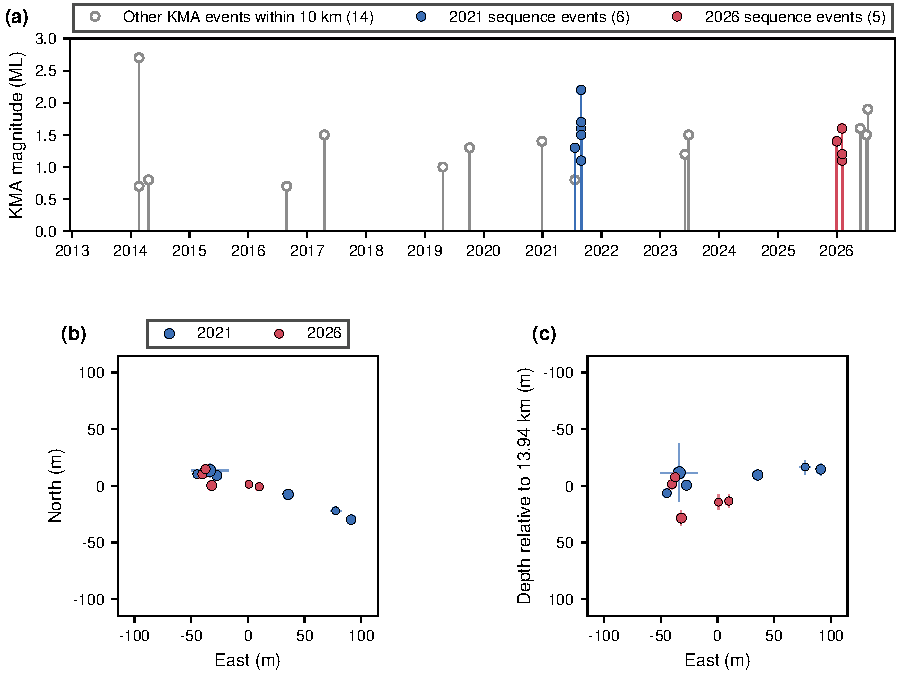
\includegraphics[width=\textwidth]{figures/Figure_01_sequence_background.pdf}
\caption{The sequence. (a) KMA-listed earthquakes within 10~km of the cluster centroid (\F{cen.lat}°~N, \F{cen.lon}°~E) since 20 December 2012 (NECIS domestic catalog, UTC): the \F{seq.n21} events of 2021 and the \F{seq.n26} of 2026 in color, the \F{kma.n10_other} others open (\F{kma.n10_other_years}). (b) Map view and (c) east--depth section of the earlier relocation of the \F{seq.n} sequence events; symbol size grows with magnitude, bars are bootstrap 95\,\% half-widths.}
\label{fig:background}
\end{figure}

\section{Approach}

The stage structure, notebooks, decision log and report pattern are those of the 2025 Imsil study. The code is copied from the current Haenam tree (the 2026 Haenam renewal), not from the Imsil tree. The Haenam tree holds the orientation rules of 11--14 October 2026, which the Imsil port predates. Of the copied files, \F{port.n_ident} are byte-identical to the Haenam files and \F{port.n_edit} carry marked edits: region values, paths, and the inventory and link rules. Detection uses the frozen Haenam settings and network weights, which were validated on the 2024 Buan sequence \citep{Seo2025}.

\textbf{Why sensor orientation matters.} A seismometer's two horizontal components are meant to point north and east. In practice the north component can point elsewhere, and the angle changes when an instrument is installed, serviced or replaced. This angle is called the \emph{misorientation}. Two steps of the study depend on it:
\begin{itemize}
\item \textbf{S-wave timing.} For relocation, S arrival-time differences between events come from cross-correlation of the horizontal records. We measure them on the \emph{transverse} component, the horizontal motion perpendicular to the source--station direction, where S is strongest and P weakest. Computing the transverse component needs the angle valid on the day of each event. A wrong angle mixes components and can bias the measured time.
\item \textbf{Template matching.} A template recorded in 2021 is compared with the records of every day from 2012 to 2026. If the sensor was turned between the two days, its north--east records no longer match.
\end{itemize}
The rules, decided for Haenam and applied here unchanged (decision P3), are:
\begin{enumerate}
\item one sensor per station for the whole period, chosen to have the fewest orientation changes (ties: broadband, then short period, then accelerometer);
\item one dated orientation table, used by every stage;
\item S differential times on the transverse component, P on the vertical;
\item template north--east windows turned into each scanned day's orientation, with the continuous data never rotated;
\item local magnitudes from every station with a valid instrument response, without station corrections.
\end{enumerate}

\section{Data}

\subsection{Stations}

The network within 100~km of the cluster holds \F{sta.n} station codes: \F{sta.n_ks} of KMA (network KS) and \F{sta.n_kg} of the Korea Institute of Geoscience and Mineral Resources (KIGAM, network KG) (\figref{fig:map}). Five temporary codes of 2023 (\F{sta.temp}) are read as their own sites. The nearest station is \F{sta.nearest}. The chosen sensors are \F{sta.n_HH} broadband (HH), \F{sta.n_EL} short-period (EL) and \F{sta.n_HG} accelerometers (HG).
The sensor rule above has one addition for a 14-year window (decision G-D1b). A sensor whose record is more than a year shorter than the station's longest is not eligible. Without it, stations such as BOSB, NAWB, HAMB and KOHB would be read on accelerometers that start only in 2016, and they would drop out of 2012--2015.
Where a station moved within 1~km and changed its code, the older code is used until the day before the newer one starts (G-D10). One code, KS.KWJ, is excluded (G-D20): its files on MARA are numbered in sequence rather than by day of year and sampled at 80~Hz, so linked by name they would put April data on 1 January.

The network grew strongly over time (\figref{fig:perYear}a). Within 60~km, \F{sta.n60_2013} stations recorded in 2013, \F{sta.n60_2016} in 2016, \F{sta.n60_2021} in 2021 and \F{sta.n60_2026} in 2026. Within 50~km the counts are \F{sta.n50_2013}, \F{sta.n50_2016}, \F{sta.n50_2021} and \F{sta.n50_2026}. Five early stations recorded only on 20-sample-per-second short-period channels until March 2015, the closest being YSU at 16.6~km. These channels have no instrument response in any metadata source and cannot carry the 5--20~Hz band of the cross-correlation. They are not used for now (G-D12, open).

\begin{figure}[t]
\centering
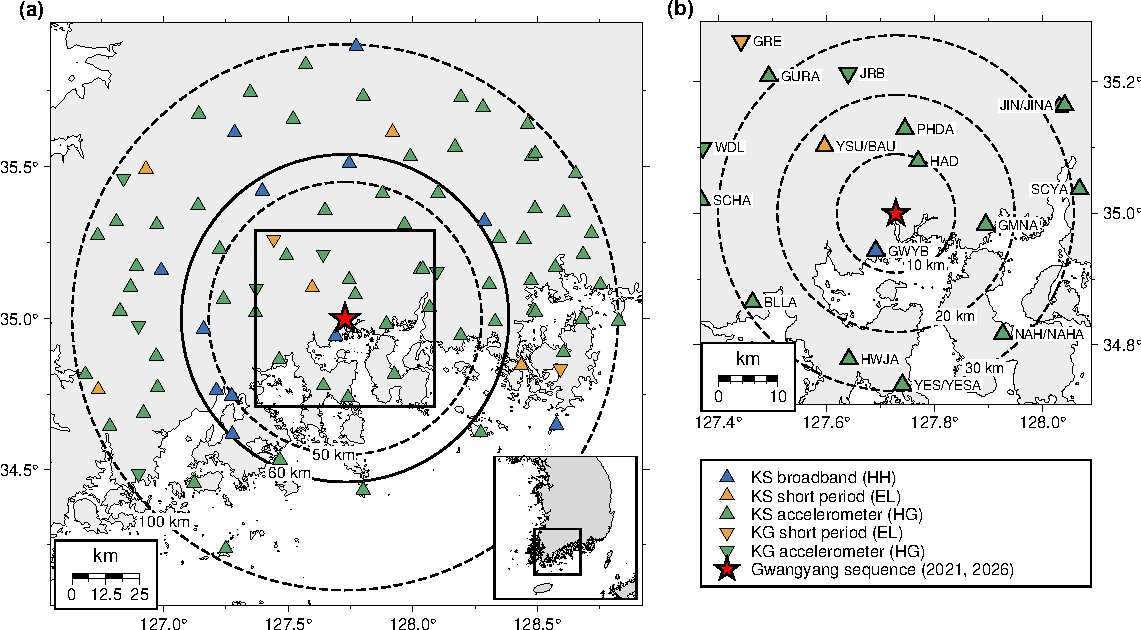
\includegraphics[width=\textwidth]{figures/Figure_02_station_map.pdf}
\caption{Stations. (a) The \F{sta.n} station codes within 100~km of the cluster (star), colored by the chosen sensor; triangles KS, inverted triangles KG. The solid circle (60~km) bounds the template-matching stations. Inset: location in Korea. (b) The box of panel (a); codes that replaced each other at one site are joined by a slash.}
\label{fig:map}
\end{figure}

\begin{figure}[t]
\centering
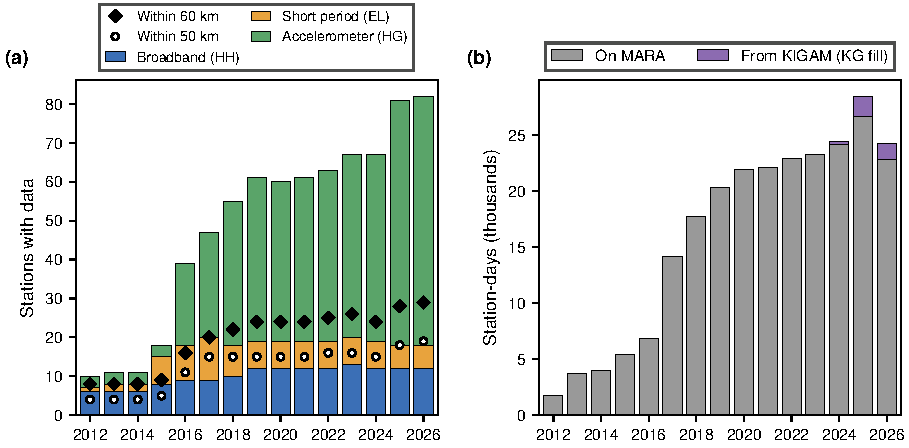
\includegraphics[width=\textwidth]{figures/Figure_03_data_per_year.pdf}
\caption{Stations and data per year. (a) Stations within 100~km with data from their chosen sensor, by sensor type; diamonds and circles count those within 60 and 50~km. (b) Station-days of the chosen sensors: on the MARA archive, and fetched from KIGAM (KG stations after October 2024). Whole calendar years are counted; the study starts on 20 December 2012.}
\label{fig:perYear}
\end{figure}

\subsection{Continuous data}

Three sources are used, each for one purpose:
\begin{itemize}
\item \textbf{MARA}, the laboratory's copy of the KMA and KIGAM archives, provides almost everything: \F{data.sd_mara} station-days of the chosen sensors, \F{stat.pull_tb}~TB, mirrored onto the analysis machine. A verification against MARA finds only files of 8 October 2026, after the window, missing.
\item \textbf{KIGAM's data service (FDSN)} provides the KG stations after 31 October 2024, where MARA ends: \F{data.sd_kigam} station-days, fetched as \F{stat.kigam_files} files with \F{stat.kigam_err} errors (G-D14). Without it, JRB, GSU and GRE, all within 40~km, would be missing from the whole 2026 episode.
\item \textbf{NECIS}, KMA's public data portal, fills only the holes in MARA (G-D13). KMA's own archive, of which MARA is a copy, lacks some channels on some days. On 2021-08-27, the day of the \ML\ 2.2, the vertical component is missing at seven nearby stations while the horizontals are present. NECIS sometimes still holds such files.
\end{itemize}
Every stage reads one tree of links to the chosen sensors' day files: \F{stat.links} links, which pass a consistency check (no dangling, misplaced or missing link).

\subsection{Completeness of the episode data}

A check of every station and day found 2026 complete. In 2021 it found \F{aud.z0} station-days with only the vertical missing, all inside the episode, and \F{aud.w0} whole station-days missing. \F{nec.rec} of \F{nec.jobs} requests to NECIS recovered files (\F{nec.files} day files), among them GWYB's vertical on 28 August and BAU's whole day on 27 August.
Over July--September 2021, \F{f4.pct}\,\% of the station-days of the \F{f4.nsta} stations are now complete (\figref{fig:complete}). \F{f4.n_nec} station-days are complete only thanks to NECIS, and \F{f4.n_part} still lack the vertical. Three of those four belong to BOSB and GMNA, two stations that have since closed and that NECIS no longer serves. Over the whole window, only \F{aud.all} station-days in 2012--2026 lack a component.

\begin{figure}[p]
\centering
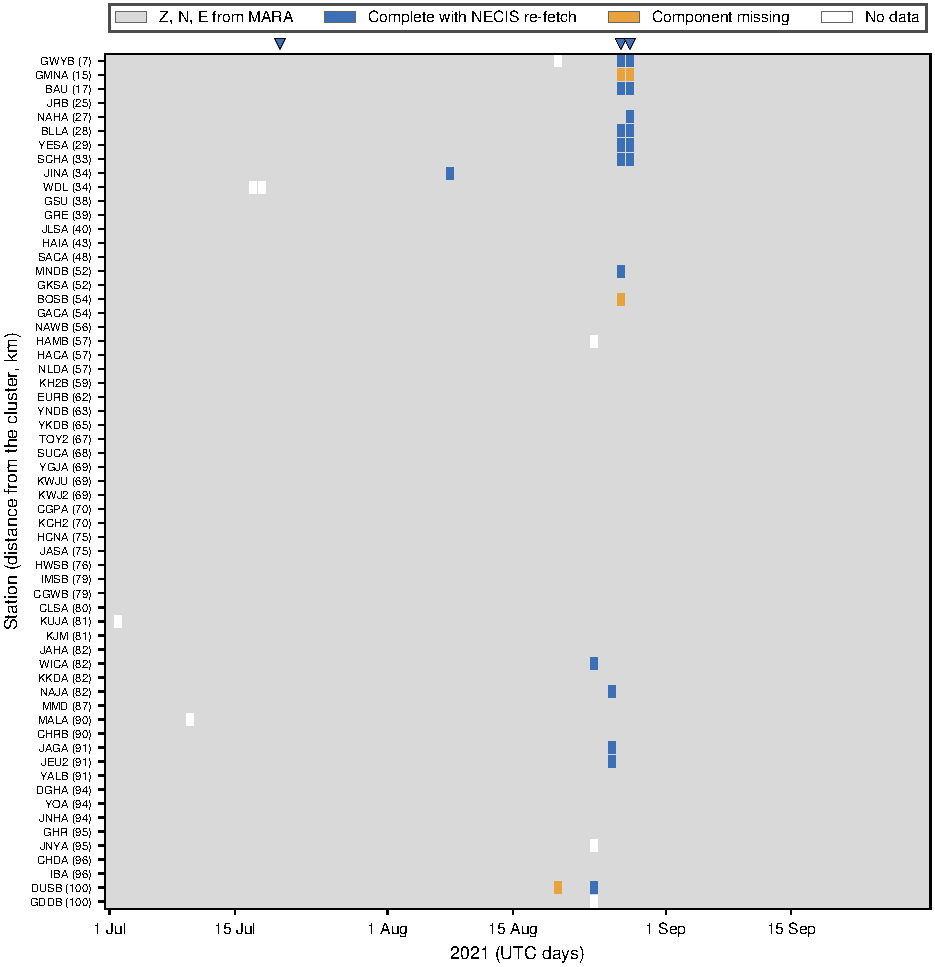
\includegraphics[width=0.94\textwidth]{figures/Figure_04_episode_2021_completeness.pdf}
\caption{Data of the 2021 episode, day by day, for the \F{f4.nsta} stations that recorded between 1 July and 30 September 2021, sorted by distance from the cluster (km in brackets). Gray: all three components from MARA; blue: complete with components re-fetched from NECIS; orange: a component missing; white: no data. Triangles: days of the KMA-listed 2021 events.}
\label{fig:complete}
\end{figure}

\FloatBarrier
\section{Sensor orientation}

\textbf{Method.} The misorientation is measured from the direction of P-wave motion of distant large earthquakes (teleseisms of magnitude 5.5 or more). A P wave moves the ground along its direction of travel, so on a correctly oriented sensor the horizontal motion points toward the source. The difference between the observed and the expected direction is the misorientation \citep{Seo2022}.
The national study of all Korean stations (`33' below) applied this method to every KS and KG station up to August--September 2026. It found the periods of constant angle, wiring faults, silent channels and gain errors. Each change is dated by a metadata epoch inside its bracket where one exists.
This study takes those tables. It measures, with the same code and settings, what they lack: the Gwangyang sensors never measured, the years before the national study's data begin, and every station to the end of the window.

\textbf{Check of the local measurement.} The national study cut its windows from KMA's waveform server; this study cuts them from the downloaded day files. On the \F{chk.n} teleseisms that both measured and both accepted, the two angles differ by a median of \F{chk.med}°, a 95th percentile of \F{chk.p95}° and at most \F{chk.max}° (\figref{fig:orient}c).

\textbf{Result.} The final run on the complete data measured \F{g2.windows} station--teleseism windows. It gives \F{g2.periods} periods of constant angle for \F{g2.units} sensors (\F{g2.valid} valid).
GWYB, 7~km from the cluster, has four periods (\figref{fig:orient}a):
\begin{itemize}
\item \F{gwyb.t1}° from \F{gwyb.s1} to \F{gwyb.e1};
\item \F{gwyb.t2}° from \F{gwyb.s2} to \F{gwyb.e2};
\item \F{gwyb.t3}° from \F{gwyb.s3} to \F{gwyb.e3};
\item \F{gwyb.t4}° from \F{gwyb.s4} to the end.
\end{itemize}
These rest on \F{gwyb.n_ev} accepted measurements. The two episodes therefore fall in different periods: 2021 in the third and 2026 in the fourth.
Of the \F{ori.n60} chosen sensors within 60~km, \F{ori.n_changed60} changed orientation at least once (\figref{fig:orient}b). Overall, \F{ori.n_meas} chosen sensors have at least one measured period. \F{ori.n_none} have none (\F{ori.none}), all short-lived accelerometers of 2016--2018. A sensor that stays unmeasured is treated as unturned and flagged (G-D2). On days inside a change bracket no transverse component is formed and the template's S windows get zero weight.

\begin{figure}[t]
\centering
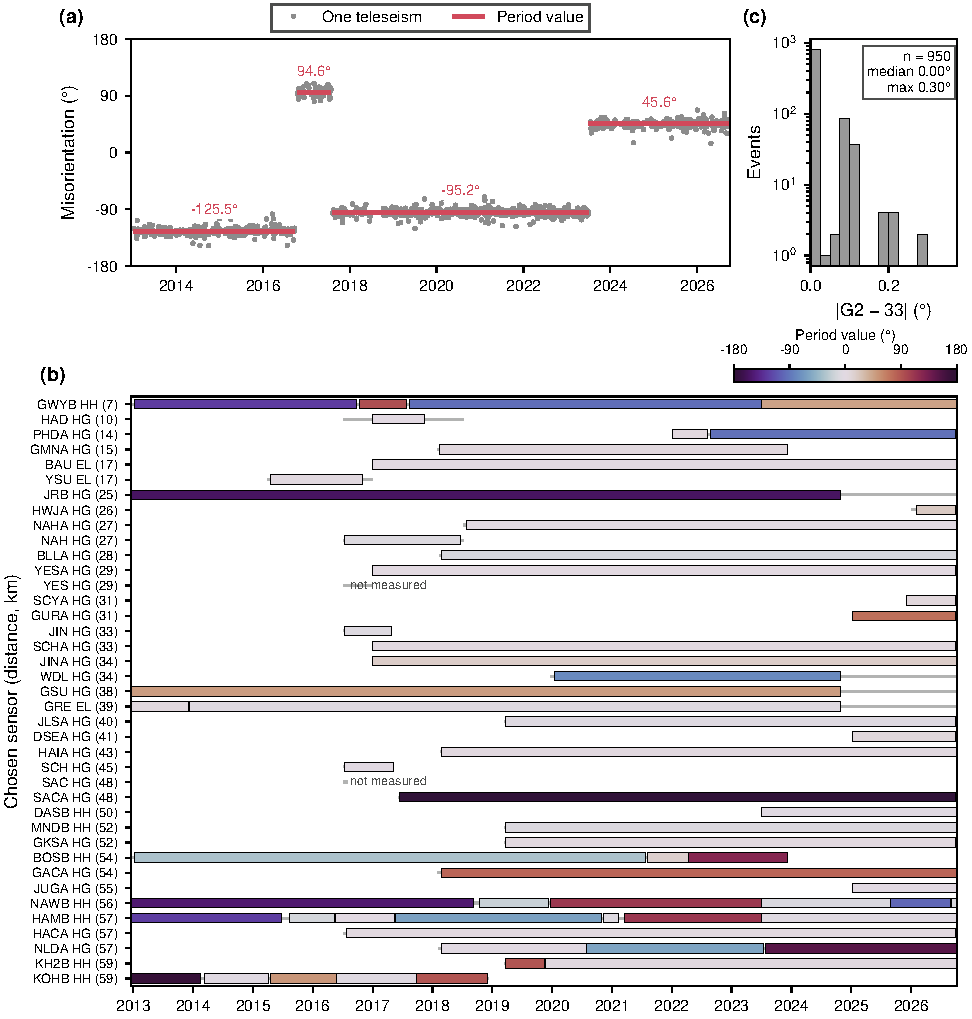
\includegraphics[width=\textwidth]{figures/Figure_05_orientation.pdf}
\caption{Sensor orientation. (a) KS.GWYB broadband: the misorientation measured on each accepted teleseism (gray) and the four period values of the orientation table (red). (b) Orientation periods of the chosen sensors within 60~km, colored by angle; thin gray lines are the data spans, and a gap between colored bars is an unresolved change bracket. (c) The same teleseisms measured from the local day files (this study, G2) and from the national study's server windows (33): absolute difference of the accepted angles.}
\label{fig:orient}
\end{figure}

\section{Processing stages}

\figref{fig:stages} and Table~\ref{tab:stages} give the ten stages. Every script runs as a dry run unless told to write, and each stage ends with a numbered notebook. That notebook holds its figures, its pass or fail lines and a computed summary. Detection, cross-correlation and template matching never share the graphics processor, neither with each other nor with other projects' jobs on the same machine.
Before production detection, a \emph{pilot} on parts of the two episode years exercised the detection code (Section~\ref{sec:pilot}). It runs in a separate folder, and no production stage reads it.

\begin{figure}[t]
\centering
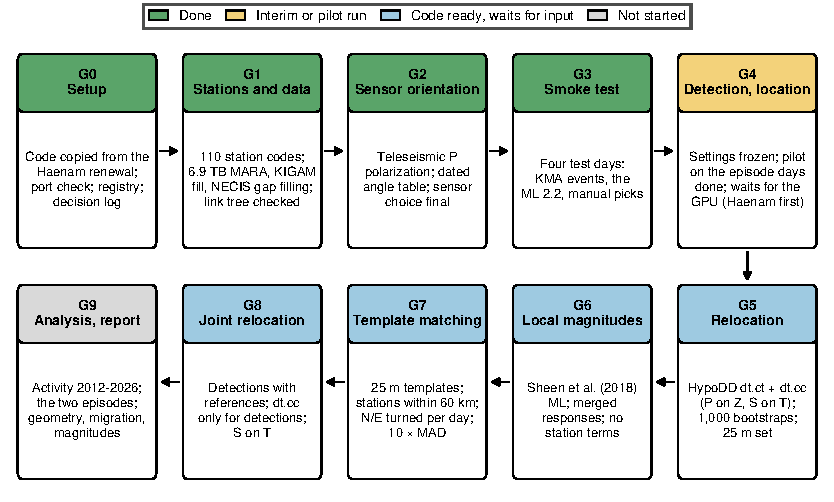
\includegraphics[width=\textwidth]{figures/Figure_06_stages.pdf}
\caption{Processing stages and their status as of \F{stat.time}.}
\label{fig:stages}
\end{figure}

\begin{table}[p]
\centering
\small
\caption{Stages, settings and checks. The detection and relocation settings are the frozen Haenam values.}
\label{tab:stages}
\begin{tabularx}{\textwidth}{@{}l>{\raggedright\arraybackslash}X>{\raggedright\arraybackslash}X@{}}
\toprule
Stage & Method and settings & Check \\
\midrule
G0 Setup & Copy of the Haenam tree with checksums; project registry of paths; decision log & port check: \F{port.n_ident} identical, \F{port.n_edit} marked edits \\
G1 Stations, data & Station inventory; MARA mirror; KIGAM fill; NECIS gap filling; one link tree of the chosen sensors & every chosen station-day audited for missing components \\
G2 Orientation & Teleseismic P polarization \citep{Seo2022}; national tables plus local measurements; one dated table; final sensor choice & local versus national angles; sensor rule applied to every multi-sensor station \\
G3 Smoke test & Full detection chain on 2021-08-27/28, 2026-01-01 and 2013-07-19 & passed: \F{smoke.kma} KMA events within \F{smoke.dtmax}~s; \ML\ 2.2 \F{smoke.epi}~km from the earlier relocation; picks within \F{smoke.dP}~s (P) and \F{smoke.dS}~s (S) of manual picks (median, \F{smoke.npk} picks) \\
G4 Detection & PhaseNet+, the multi-task successor of PhaseNet \citep{Zhu2019}, at \F{p.fs}~Hz, probability $\ge$\,\F{p.pmin}; association with PyOcto \citep{Munchmeyer2024}, $\ge$\,\F{p.n_picks} picks ($\ge$\,\F{p.n_p} P, $\ge$\,\F{p.n_s} S) in \F{p.box_lat}, \F{p.box_lon}; HYPOINVERSE \citep{Klein2002} in the model of \citet{KimKim1983} & all \F{kma.n5} KMA events within 5~km and the other KMA events within 10~km; regional KMA recovery; activity per year \\
G5 Relocation & Events within \F{p.radius}~km of the centroid, depth $\ge$\,10~km, gap $<$\,\F{p.gap}°, $>$\,\F{p.num} phases, RMS $<$\,\F{p.rms}~s, errors $<$\,\F{p.err}~km; double difference \citep{Waldhauser2000} with catalog and cross-correlation times (\F{p.xc_band}~Hz, $\pm$\F{p.xc_win}~s, \F{p.xc_interp}~Hz interpolation, CC $\ge$\,\F{p.xc_cc}, $\ge$\,\F{p.obscc} per pair), P on the vertical and S on the transverse; \F{prev.nboot} bootstrap replicas; \emph{reference set} = events with 95\,\% half-widths $\le$\,25~m in east, north and depth; plane fitted to the reference events within 1~km of the \ML\ 2.2 & relative positions against the earlier relocation after one rigid shift; S on the transverse against north--east at stations that never turned; how links survive across instrument changes \\
G6 Magnitudes & \citet{Sheen2018} scale; every station with a valid response on the event day (merged metadata of KMA, KIGAM and NECIS); signal-to-noise $\ge$\,\F{p.ml_snr}; $\ge$\,\F{p.ml_nsta} picked stations; no station corrections & our \ML\ against KMA \ML\ for the listed events \\
G7 Template matching & Templates = reference set; stations within 60~km, one sensor each; \F{p.fmf_band}~Hz; \F{p.fmf_win}~s windows from \F{p.fmf_pre}~s before P (vertical) and S (north, east); template north--east turned into each day's orientation; per-channel signal-to-noise $\ge$\,\F{p.fmf_snr}; detection $\ge$\,\F{p.fmf_mad} times the median absolute deviation of the network correlation, per station configuration, with $\ge$\,\F{p.fmf_minsta} stations \citep{Beauce2018} & self-detection of every template; GWYB templates detected in all four orientation periods; the Haenam threshold (12 times plus a correlation floor of 0.2) compared on the episode days; evidence notebooks for noise bursts and single-template families \\
G8 Joint relocation & New detections inherit their template's picks (only to place the windows) and enter by cross-correlation times alone, with the references; S on the transverse; G5 settings, bootstrap and 25~m rule & reference events move little; detection pass rate versus correlation \\
G9 Analysis, report & Activity history by episode; repeat or neighbor; plane; migration; magnitudes and completeness per network era; report with the same fact system & answers to Q1--Q5 with uncertainties \\
\bottomrule
\end{tabularx}
\end{table}

\FloatBarrier
\section{Pilot results on the episode days}
\label{sec:pilot}

The pilot ran the frozen detection chain on 2021 days \F{pilot.days21} and on 2026 days \F{pilot.days26}, with the station table from before the freeze (no KG stations in 2026). The relocation selection of G5 keeps \F{pilot.n} events: \F{pilot.n_seq} on the KMA sequence list, \F{pilot.n_kmao} other KMA-listed event (\F{pilot.kmao}) and \F{pilot.n_new} not in the KMA catalog. Appendix~\ref{app:pilot} lists them all. These are single-event HYPOINVERSE locations; the cross-correlation relocation comes with the production run (G5).
KMA lists \F{kma.n5} events within 5~km of the patch since December 2012, three more than the sequence list. The production detection is checked against all of them (decision R5).

\textbf{Locations.} The KMA-listed events locate with a median of \F{pilot.q_kma}; the new events with \F{pilot.q_new} (\figref{fig:pilotrel}, \figref{fig:pilotabs}). The median largest principal 1$\sigma$ error is \F{pilot.e1_kma}~km for the KMA-listed events and \F{pilot.e1_new}~km for the new ones. The \F{pilot.n_poor} new events with 12 or fewer phases or a vertical error above 1~km come out shallower and off the patch, with error ellipses elongated toward the surface. A double-difference relocation from the picks alone already draws \F{pilot.dd_n} of the events together to standard deviations of \F{pilot.dd_std}, against \F{pilot.hyp_std} east, north and in depth for HYPOINVERSE.

\textbf{Same patch?} Two tests do not depend on the locations (\figref{fig:pilotwave}, \figref{fig:pilotsame}).
\begin{itemize}
\item \textbf{S$-$P intervals.} At a given station, events at the same place have the same S$-$P interval. \F{pilot.n_samesp} of the \F{pilot.n_new} new events match the KMA events within 0.1~s (about 0.8~km) at every station with both picks.
\item \textbf{Waveforms.} At the stations where they have signal, \F{pilot.n_noise} correlate with the \ML\ 2.2 above the noise baseline (\F{pilot.noiseP} for P, \F{pilot.noiseS} for S). \F{pilot.n_cc07} reach the relocation threshold of 0.7.
\end{itemize}
\F{pilot.fail} fail: the first comes from elsewhere (a shorter S$-$P interval, a location a few kilometers away and deeper); the second is too weak to decide. Template matching and the relocation decide such cases with more stations.

\textbf{Size.} Relative magnitudes come from S-wave amplitude ratios (5--20~Hz) against the KMA events of the same year. Left out one at a time, the KMA events are reproduced with an RMS difference of \F{pilot.loo_rms} (\F{pilot.loo21} in 2021, \F{pilot.loo26} in 2026). The new events are \F{pilot.ml_new} (median \F{pilot.ml_new_med}), below the KMA events (\figref{fig:pilotmag}). The 2021 values rest on about \F{pilot.n_amp21} stations each and may be low by up to \F{pilot.low21}.

\textbf{Timing} (\figref{fig:pilottime}). \F{pilot.pre20_n} new events (\F{pilot.pre20}) preceded the first KMA-listed event of 2021 by \F{pilot.pre20_lead}~days. Their S$-$P intervals match within \F{pilot.pre20_sp}~s, and their S waves correlate with the \ML\ 2.2 at \F{pilot.pre20_cc}. \F{pilot.pre27_n} more (\F{pilot.pre27} on 26 August) preceded the 27 August events, and \F{pilot.post26_n} (\F{pilot.post26}) followed the last KMA-listed event of the 2026 episode. The KMA-listed event of 26 May 2026 lies on the patch after the second episode. The pilot covered only parts of the two years; production detection over the whole window (G4) and template matching (G7) will show whether activity started earlier and how often the patch was active between the episodes (Q1).

\begin{figure}[t]
\centering
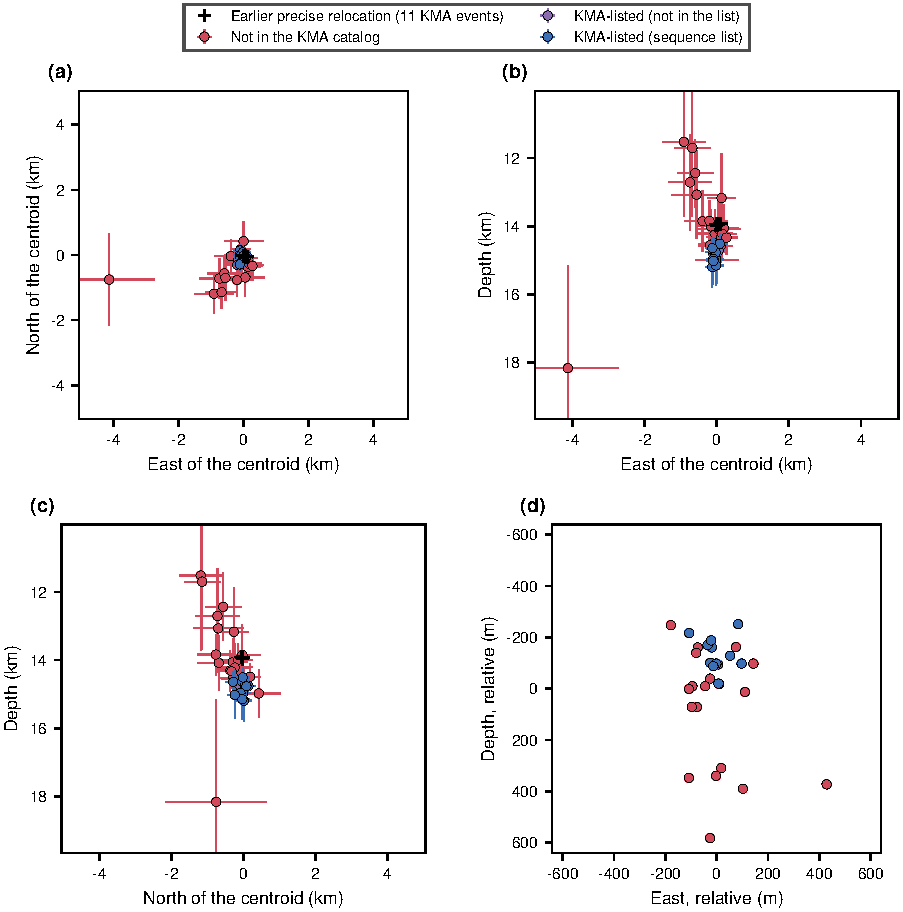
\includegraphics[width=\textwidth]{figures/Figure_07_pilot_locations_relative.pdf}
\caption{Pilot events, relative view. (a) Map view and (b, c) depth sections of the HYPOINVERSE locations in km from the cluster centroid, with HYPOINVERSE errors (ERH horizontally, ERZ vertically). Black crosses: the earlier precise relocation of the 11 sequence events. (d) Double-difference relocation from the picks alone, relative to its mean.}
\label{fig:pilotrel}
\end{figure}

\begin{figure}[t]
\centering
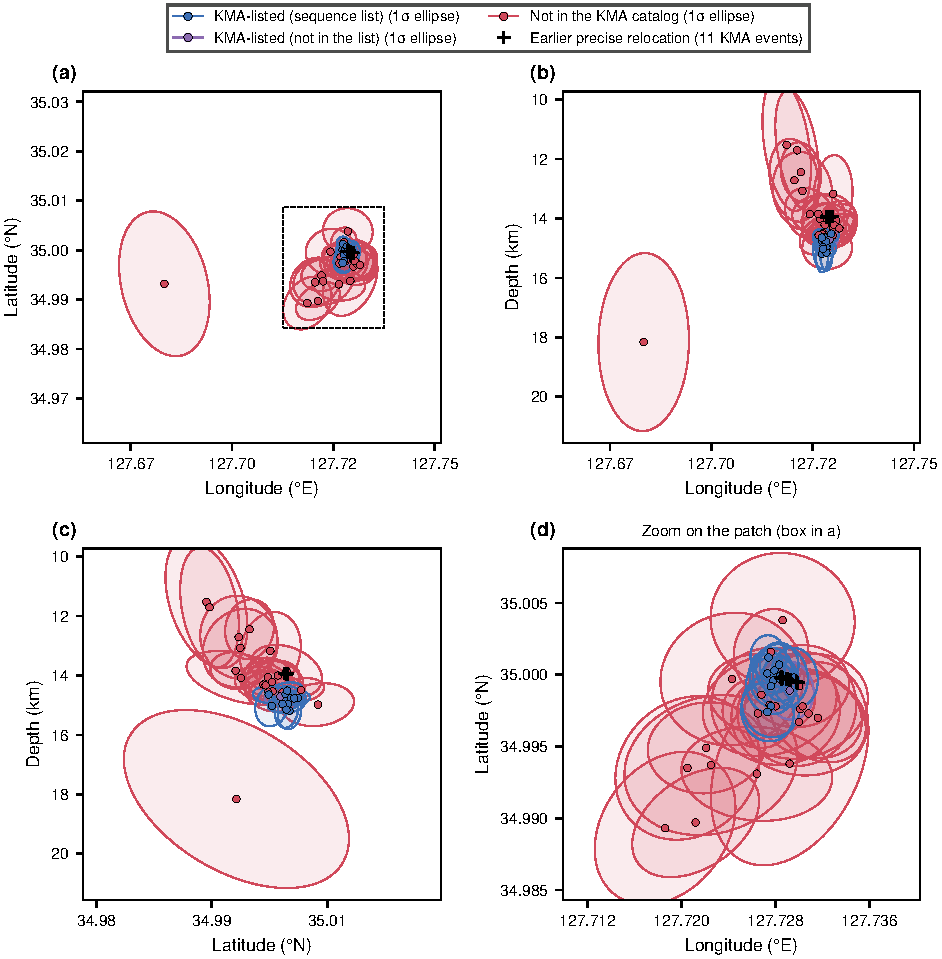
\includegraphics[width=\textwidth]{figures/Figure_08_pilot_locations_absolute.pdf}
\caption{Pilot events, absolute view: HYPOINVERSE locations with 1$\sigma$ error ellipses (the three principal error axes of each event, from HYPOINVERSE's archive file, projected onto each plane). Black crosses: the earlier precise relocation. (d) Zoom on the patch (box in a).}
\label{fig:pilotabs}
\end{figure}

\begin{figure}[p]
\centering
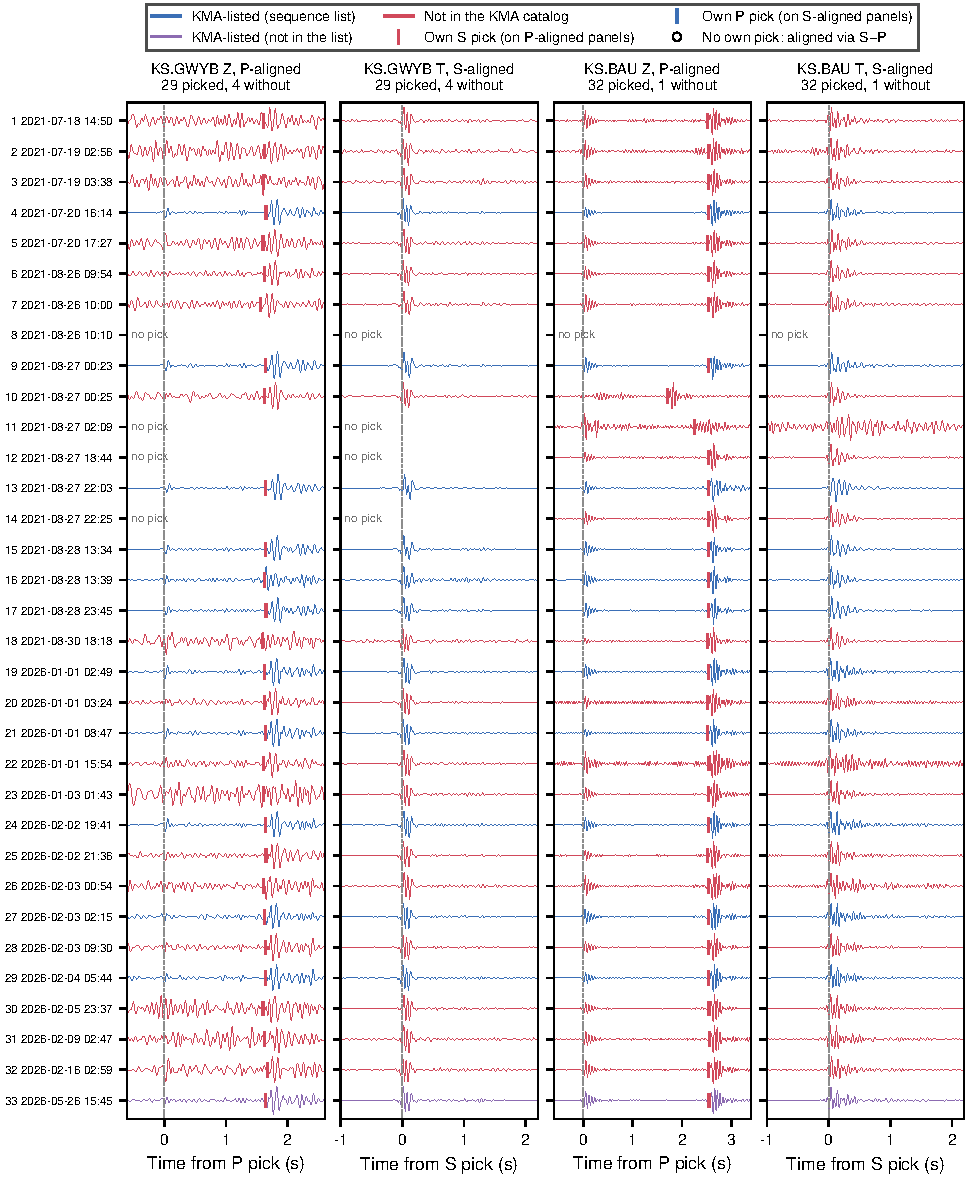
\includegraphics[width=\textwidth]{figures/Figure_09_pilot_waveforms.pdf}
\caption{Waveforms of the \F{pilot.n} pilot events at KS.GWYB (7~km) and KS.BAU (17~km), 5--20~Hz, normalized. Vertical components are aligned on each event's own P pick, transverse components on its own S pick; ticks mark the other pick, so that equal S$-$P intervals line up. Events without a pick at a station are labeled.}
\label{fig:pilotwave}
\end{figure}

\begin{figure}[t]
\centering
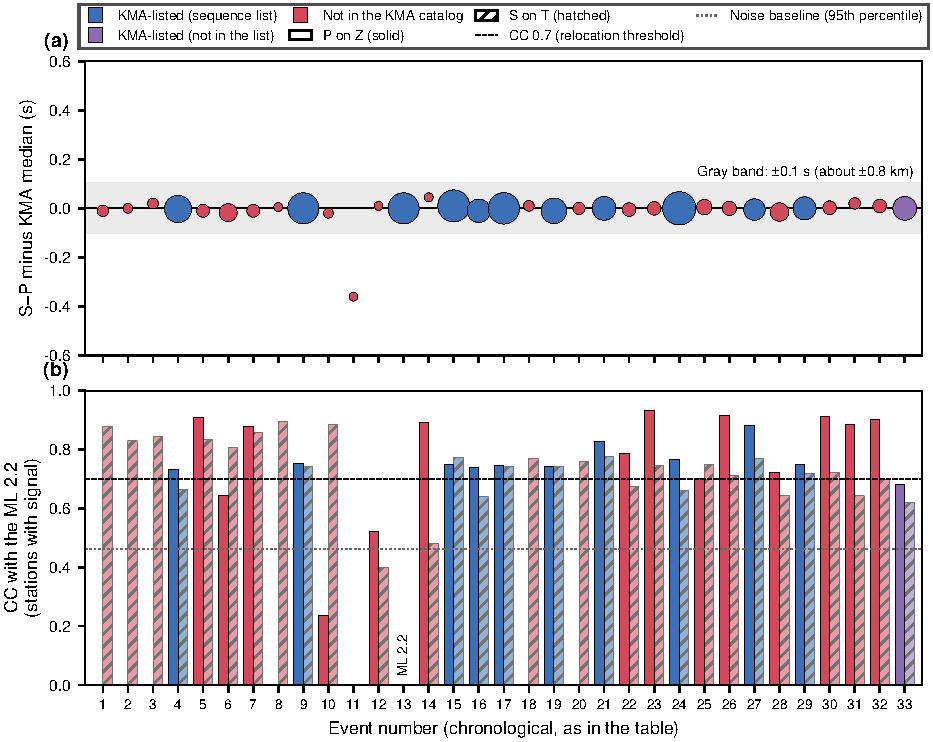
\includegraphics[width=\textwidth]{figures/Figure_10_pilot_same_patch.pdf}
\caption{Are the pilot events on the same patch? (a) Each event's S$-$P interval minus that of the KMA events at the same station (median over the stations with both picks; symbol size grows with the number of stations); gray band $\pm$0.1~s. (b) Cross-correlation with the \ML\ 2.2 (5--20~Hz) at the stations where the event has signal, median over those stations; P on the vertical solid, S on the transverse hatched. Dashed: the relocation threshold; dotted: the noise baseline.}
\label{fig:pilotsame}
\end{figure}

\begin{figure}[t]
\centering
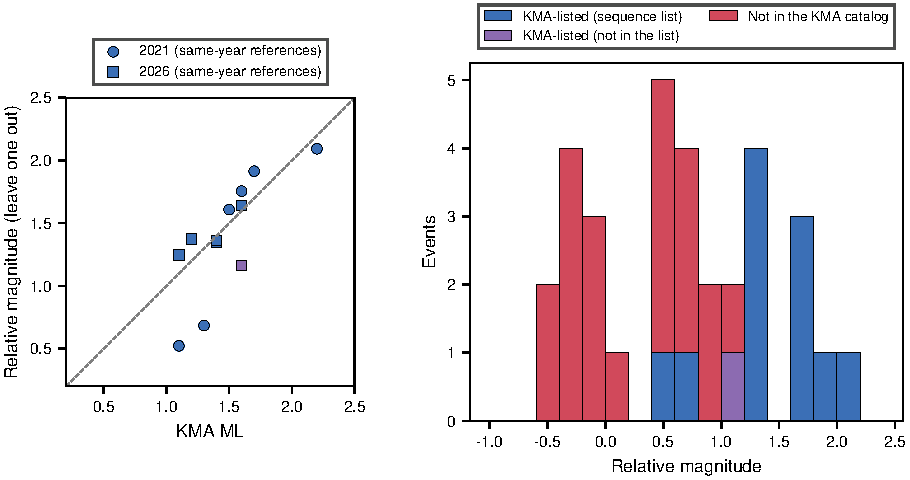
\includegraphics[width=\textwidth]{figures/Figure_11_pilot_magnitudes.pdf}
\caption{Relative magnitudes from S-wave amplitude ratios. (a) Each KMA-listed event estimated from the other KMA-listed events of the same year, against its KMA \ML. (b) Distribution for all \F{pilot.n} pilot events.}
\label{fig:pilotmag}
\end{figure}

\begin{figure}[t]
\centering
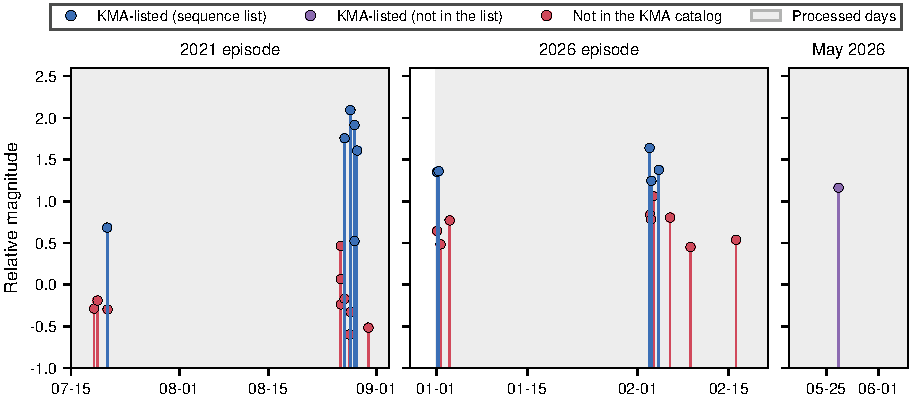
\includegraphics[width=\textwidth]{figures/Figure_12_pilot_timeline.pdf}
\caption{The pilot events in time, each episode on its own axis; processed days shaded.}
\label{fig:pilottime}
\end{figure}

\FloatBarrier
\section{Independent checks}
\label{sec:checks}

A check counts only if it does not reuse the quantity being fitted. The study uses:
\begin{enumerate}
\item recovery of the KMA-listed events: the \F{kma.n5} events within 5~km (the \F{seq.n} of the sequence list and three more, decision R5), the other events within 10~km, and the regional catalog;
\item the earlier relocation: after one rigid shift, the relative positions of the \F{prev.n} sequence events should agree within their uncertainties;
\item S-wave times on the transverse component against those on north and east, at stations whose orientation never changed: they should agree to about 1~ms;
\item GWYB templates of 2021 found again on days in each of GWYB's four orientation periods, which tests the turning of the templates;
\item every template detecting its own event;
\item the local versus the national orientation measurements (done: median difference \F{chk.med}°);
\item the smoke test of the detection chain (done, Table~\ref{tab:stages}).
\end{enumerate}

\section{Status and schedule}

At \F{stat.time}, stages G0--G3 are complete.
\begin{itemize}
\item \textbf{Downloads.} MARA: all \F{stat.pull_tot} station-sensor-years, \F{stat.pull_tb}~TB, no problems. KIGAM: \F{stat.kigam_files} files, \F{stat.kigam_err} errors. NECIS gap filling done.
\item \textbf{Inputs.} The link tree holds \F{stat.links} links. The final orientation run and the final sensor choice are done.
\item \textbf{Freeze.} The detection parameters were frozen at \F{stat.freeze_time} (hash \F{stat.freeze}).
\end{itemize}
Production detection (G4) needs moho's graphics processor. The Haenam template-matching scan holds it; the Haenam work has priority, and the scan should end around 19 October. Then, in order:
\begin{enumerate}
\item a short run of the pilot relocation on the graphics processor, to check the cross-correlation stage on the \F{pilot.n} pilot events;
\item production detection over all years: about two days with four chains, at the Haenam rate of about 2.75~s per station-day per chain;
\item relocation (G5) and magnitudes (G6);
\item template matching (G7), timed on the episode days first; about five days at the Haenam rate of about 1.5~min per day;
\item the joint relocation (G8) and the analysis (G9).
\end{enumerate}

\section{Risks and limitations}

\begin{itemize}
\item \textbf{A changing network.} With \F{sta.n60_2013} stations within 60~km in 2013 against \F{sta.n60_2021} in 2021, detection is less sensitive in the early years. Activity before 2016 can only be compared with later activity above an era-specific completeness magnitude (Q5).
\item \textbf{Links across instrument changes.} Cross-correlation needs similar waveforms. A sensor replaced between two events lowers the correlation, so early events may be tied to the later ones by fewer measurements. This is reported per era.
\item \textbf{Orientation gaps.} On days inside a change bracket, or at a sensor never measured, S is not measured on the transverse component and the template's S windows get no weight. After the final orientation run, \F{ori.n_none} chosen sensors remain unmeasured, all short-lived accelerometers of 2016--2018.
\item \textbf{Shared graphics processor.} Gwangyang's GPU stages run only when the GPU is free of the higher-priority Haenam work, so the schedule follows Haenam's.
\item \textbf{Data holes.} The vertical components still missing on the \ML\ 2.2 days (BOSB, GMNA) and the HWJA outage of January--May 2026 cannot be filled.
\item \textbf{False detections over 14 years.} Long template-matching scans pick up noise bursts and events seen by a single template. Each candidate group is vetted in its own notebook, as for Imsil.
\item \textbf{Open decisions:} \F{dec.open} (Appendix~\ref{app:decisions}). G-D12 is the use of the early 20-sample-per-second channels; G-D19 is the list of templates excluded from the catalog, which is re-derived when the templates exist.
\end{itemize}

\section{Deliverables}

\begin{itemize}
\item catalogs: the detection catalog 2012--2026; the relocated catalog with its 25~m reference set and fault plane; local magnitudes; the template-matching catalog; the joint relocation of the detections;
\item stage notebooks 00--10, each with figures, checks and a computed summary, and the decision log;
\item a results report built like this one, in which every number comes from a notebook;
\item on request, a public code repository with server names and credentials removed, as for Imsil.
\end{itemize}

\FloatBarrier
\bibliographystyle{plainnat}
\bibliography{refs}

\clearpage
\appendix
\section{Decision log}
\label{app:decisions}

All settings of this study as recorded in \texttt{docs/decisions.csv} (\F{dec.n} rows, \F{dec.n_gd} of them Gwangyang decisions G-D). P: decided before the work started; R: region values set by rule; G-D: settings this study had to choose, with the evidence in the log. Status \emph{default} means the plan's default, applied because the stages run unattended; such a setting can be changed on review.

{\footnotesize
% written by notebooks/90_study_plan_report.ipynb from docs/decisions.csv; do not edit by hand
\begin{longtable}{@{}p{1.0cm}>{\raggedright\arraybackslash}p{3.4cm}>{\raggedright\arraybackslash}p{8.6cm}p{1.8cm}@{}}
\toprule
ID & Setting & Gwangyang value & Status \\
\midrule
\endhead
P1 & study window & 2012-12-20 (first KS.GWYB day) .. 2026-10-06 (last day on MARA, 2026-10-15 listing) & decided \\
P2 & machine and project folder & moho /home/msseo/works/73.Gwangyang\_sequence & decided \\
P3 & method rules & the same: one sensor per station, one dated orientation table, S dt.cc on T, template N/E turned to each scanned day, ML without station terms & decided \\
P4 & networks & KS + KG where data exist; JU not used & decided \\
R1 & association box & 34.30-35.70 N, 126.93-128.53 E & rule \\
R2 & source centroid & 35.0000 N 127.7286 E & rule \\
R3 & relocation selection & within 5 km of 35.0000 N 127.7286 E, depth $\geq$ 10 km, same quality gate (relocation\_selection.py) & rule \\
R4 & station set & 115 KS/KG codes within 100 km with data in the window (107 KS, 8 KG; 5 of them temporary codes of 2023; KS.KWJ excluded, G-D20) & rule \\
R5 & known events & registry/events.csv: the 11 KMA events of the two episodes (UTC); all 14 KMA events within 5 km in the window (NECIS catalog to 2026-10-13) are the G4 recovery check & rule \\
G-D1 & sensor per station & the sensor rule for every multi-sensor station (after the final G2 run of 2026-10-16 it applies everywhere; GWYBT and NAWBT resolved); no choice changed by G2: HG 85, HH 16, EL 14 (temporary codes included) & default \\
G-D1b & sensor rule over a 14-year window: coverage first & a sensor whose data period is > 365 d shorter than the station's longest sensor is not eligible; the discontinuity rule decides among the rest & default \\
G-D2 & unmeasured orientation spans & the same; G2 measures the gaps it can (GWYB 2012-12..2013-01, KS HG 2016-2017, after the national table ends) & default \\
G-D3 & relocation depth floor & 10 km & default \\
G-D4 & template-matching station subset & within 60 km (the plan default), one sensor each; temporary codes read as their site; template\_matching/stations\_G7\_60km.csv & default \\
G-D5 & mirror bandwidth & 8 jobs, rsync bwlimit 25 MB/s each, one ssh connection per job; measured total about 59 MB/s (the MARA-moho link limit) & default \\
G-D6 & template-matching threshold & 10 x MAD per configuration segment, no floor (Imsil D23); compared on the 2021 and 2026 days before the long scan & default \\
G-D7 & temporary codes (2023: GWYBT, NAWBT, SUCAT, DAYAT, GEJAT) & merged: linked only on days the site's chosen sensor lacks & default \\
G-D8 & KG after 2024-10-31 & superseded by G-D14 (KIGAM FDSN fill of the chosen KG sensors) & superseded \\
G-D10 & predecessor codes at one site & older code linked until the day before its successor starts (11 codes); KWJU and KWJ2 both used (renewal decision B) & default \\
G-D11 & KG stations also filed under KS on MARA (2017) & KG used; the KS copies (GRE, GSU, HDB, JRB, MUN, YSB) ignored & rule \\
G-D12 & 20 Hz SL channels (YSU, TOY, KCH, MAS, JEU before 2015-04; GRE, KJM) & not used: the frozen PhaseNet+ runs at 100 Hz and the 5-20 Hz cross-correlation band exceeds SL's 10 Hz Nyquist & open \\
G-D13 & station-days with a missing component on MARA & audit every chosen station-day after the pull; re-fetch from NECIS for the 2021 and 2026 episode days (KMA source archive gaps); elsewhere the components present are used, as the frozen pipeline does & default \\
G-D14 & KG data after 2024-10-31 & the same tool, only the chosen sensor of each KG station (station table Sensor): JRB, WDL, GSU (HG) and GRE, KJM (EL) 2024-11-01..2026-10-06; HWSB, GHR, IBA (HG) only 2026-10-01..10-06, as MARA holds them through 2026-09-30 (the Haenam R1a fill delivered to MARA) & default \\
G-D15 & template-matching scan settings other than the threshold & the same; period 2012-12-20..2026-10-06; templates = focused 25 m set of the G5 run (catalogs/templates/build\_template\_catalog.py); picks from that run only & default \\
G-D16 & 25 m reference adoption & the same definitions anchored on the 2021 ML 2.2 (2021-08-27 22:03:22 UTC); eras before 2021 / 2021 episode (Jul-Sep) / interval / 2026 episode (Jan-Feb) / after & default \\
G-D17 & NAHA in the local magnitudes & NAHA kept: the station table carries its corrected site (34.8167 N, 127.9261 E), and the SAC exports take station coordinates from the station table & default \\
G-D18 & joint relocation of the template-matching detections (G8) & Imsil D22 with S on T (R/T exported at each detection origin), each detection exported with the station table of its own year, and the G5 onset window for the 2021 ML 2.2 when it is a reference & default \\
G-D19 & templates excluded from the template-matching catalog & re-derived at G7 with the same test on the Gwangyang templates; empty until then & open \\
G-D20 & station codes excluded for unusable data & KS.KWJ excluded from the inventory and station table & default \\
G1 & data (result) & MARA pull 717,147 files (6,274.6 GB) + coverage-first supplement 64,336 files (620.7 GB), 0 problems; verify: only 2026-10-08 missing (after the window); KIGAM 10,629 files, 0 errors; NECIS 9 of 11 gap requests recovered; link tree 711,715 links, check PASS & result \\
G2 & orientation (result) & 22,078 station-teleseism windows measured from local day files; 147 P\_minT periods for 110 sensors (144 valid); local vs national: 950 events accepted by both, |diff| median 0.00, 95\% 0.10, max 0.30 deg; 6 chosen sensors unmeasured (YES, SAC, HAC, JAS, JAH, CHR: accelerometers of 2016-2018) & result \\
G3 & smoke test (2021-08-27/28, 2026-01-01, 2013-07-19) & PASS: 7/7 KMA events within 1.23 s; ML 2.2 0.12 km from the earlier relocation (depth 15.2 km HYPOINVERSE); PhaseNet+ - manual median |dt| P 0.019 s, S 0.020 s (n 458) & result \\
G4-freeze & detection parameter freeze & hash d724acfddcd608dd (config, core, pick augmentation, station table of 115 codes, PhaseNet+ weights sha f1643330...), 2026-10-16 12:51; smoke-test outputs moved to detection/smoke\_G3\_20261015 & result \\
G6-resp & merged response inventory (result) & docs/response\_inventory/merged\_inventory.xml: 636 channel epochs in 115 stations; 692,785 of 706,261 channel-days covered (98.1 percent); both episodes without a day lacking a response (2021: 61 streams, 2026: 82); 1,770 channel-days without response (station starts before their metadata in early 2018, YSU 2016, SCYA 2025-12, HAMA 2024-01..03); KWJU excluded (neither source fits its data, as in Haenam); remove\_response spot checks at 5 channels give ratios 0.998-1.001 & result \\
\bottomrule
\end{longtable}

}

\section{Pilot events}
\label{app:pilot}

The \F{pilot.n} events of the pilot (notebook 91). Origin, location, phases used (Ph.), azimuthal gap and errors from HYPOINVERSE. $\Delta$(S$-$P): median difference between the event's S$-$P intervals and those of the KMA events at the same stations. CC$_\mathrm{S}$: median correlation of the S wave with the \ML\ 2.2 at the stations where the event has signal. Rel.~M: relative magnitude. Class: KMA (sequence list), KMA* (KMA-listed, not on the list), new.

{\scriptsize\setlength{\tabcolsep}{3.2pt}
% written by notebooks/91_pilot_episode_events.ipynb; do not edit by hand
\begin{longtable}{@{}rlrrrrrrrrrrrl@{}}
\toprule
No. & Origin (UTC) & Lat. & Lon. & Depth & Ph. & Gap & ERH & ERZ & $\Delta$(S$-$P) & CC$_\mathrm{S}$ & Rel. M & KMA ML & Class \\
 & & (°N) & (°E) & (km) & & (°) & (km) & (km) & (s) & & & & \\
\midrule
\endhead
1 & 2021-07-18 14:50:01 & 34.9978 & 127.7280 & 14.21 & 15 & 86 & 0.5 & 0.7 & −0.01 & 0.88 & −0.3 &  & new \\
2 & 2021-07-19 02:56:11 & 34.9935 & 127.7205 & 12.71 & 9 & 111 & 0.6 & 1.4 & 0.00 & 0.83 & −0.2 &  & new \\
3 & 2021-07-19 03:38:12 & 34.9997 & 127.7243 & 13.85 & 12 & 109 & 0.5 & 0.9 & +0.02 & 0.84 & −0.2 &  & new \\
4 & 2021-07-20 16:14:18 & 34.9996 & 127.7278 & 14.63 & 86 & 35 & 0.2 & 0.3 & 0.00 & 0.66 & 0.7 & 1.3 & KMA \\
5 & 2021-07-20 17:27:05 & 34.9949 & 127.7221 & 12.44 & 16 & 103 & 0.5 & 1.0 & −0.01 & 0.83 & −0.3 &  & new \\
6 & 2021-08-26 09:54:43 & 35.0016 & 127.7276 & 14.49 & 43 & 40 & 0.3 & 0.4 & −0.02 & 0.81 & 0.5 &  & new \\
7 & 2021-08-26 10:00:25 & 34.9976 & 127.7301 & 13.17 & 19 & 86 & 0.4 & 1.3 & −0.01 & 0.86 & 0.1 &  & new \\
8 & 2021-08-26 10:10:18 & 35.0038 & 127.7286 & 14.98 & 10 & 86 & 0.6 & 0.7 & +0.01 & 0.90 & −0.2 &  & new \\
9 & 2021-08-27 00:23:15 & 35.0012 & 127.7274 & 14.76 & 114 & 35 & 0.2 & 0.2 & 0.00 & 0.74 & 1.8 & 1.6 & KMA \\
10 & 2021-08-27 00:25:42 & 34.9938 & 127.7292 & 14.08 & 12 & 112 & 0.6 & 0.8 & −0.02 & 0.89 & −0.2 &  & new \\
11 & 2021-08-27 02:09:29 & 34.9932 & 127.6833 & 18.16 & 8 & 140 & 1.4 & 3.0 & −0.36 &  &  &  & new \\
12 & 2021-08-27 18:44:02 & 34.9893 & 127.7186 & 11.52 & 8 & 113 & 0.6 & 2.2 & +0.01 & 0.40 & −0.6 &  & new \\
13 & 2021-08-27 22:03:23 & 35.0001 & 127.7273 & 15.19 & 114 & 35 & 0.2 & 0.6 & 0.00 &  & 2.1 & 2.2 & KMA \\
14 & 2021-08-27 22:25:31 & 34.9897 & 127.7212 & 11.70 & 10 & 108 & 0.5 & 2.0 & +0.04 & 0.48 & −0.3 &  & new \\
15 & 2021-08-28 13:34:11 & 35.0003 & 127.7279 & 14.75 & 115 & 35 & 0.2 & 0.2 & +0.01 & 0.77 & 1.9 & 1.7 & KMA \\
16 & 2021-08-28 13:39:22 & 34.9999 & 127.7284 & 14.97 & 71 & 39 & 0.2 & 0.3 & −0.01 & 0.64 & 0.5 & 1.1 & KMA \\
17 & 2021-08-28 23:45:56 & 35.0007 & 127.7283 & 14.77 & 114 & 35 & 0.2 & 0.2 & 0.00 & 0.74 & 1.6 & 1.5 & KMA \\
18 & 2021-08-30 18:18:23 & 34.9937 & 127.7225 & 13.07 & 9 & 111 & 0.7 & 1.3 & +0.01 & 0.77 & −0.5 &  & new \\
19 & 2026-01-01 02:49:47 & 34.9992 & 127.7276 & 14.96 & 82 & 40 & 0.2 & 0.3 & −0.01 & 0.74 & 1.4 & 1.4 & KMA \\
20 & 2026-01-01 03:24:59 & 34.9967 & 127.7300 & 14.31 & 17 & 70 & 0.4 & 0.6 & 0.00 & 0.76 & 0.6 &  & new \\
21 & 2026-01-01 08:47:59 & 34.9998 & 127.7296 & 14.51 & 78 & 40 & 0.2 & 0.3 & 0.00 & 0.78 & 1.4 & 1.4 & KMA \\
22 & 2026-01-01 15:54:00 & 34.9973 & 127.7308 & 14.06 & 23 & 41 & 0.4 & 0.7 & 0.00 & 0.67 & 0.5 &  & new \\
23 & 2026-01-03 01:43:12 & 34.9979 & 127.7275 & 14.53 & 20 & 70 & 0.4 & 0.7 & 0.00 & 0.75 & 0.8 &  & new \\
24 & 2026-02-02 19:41:19 & 34.9997 & 127.7284 & 15.15 & 127 & 35 & 0.2 & 0.6 & 0.00 & 0.66 & 1.6 & 1.6 & KMA \\
25 & 2026-02-02 21:36:20 & 34.9992 & 127.7300 & 14.57 & 30 & 54 & 0.3 & 0.5 & +0.01 & 0.75 & 0.8 &  & new \\
26 & 2026-02-03 00:54:43 & 34.9986 & 127.7268 & 14.00 & 26 & 50 & 0.4 & 0.5 & 0.00 & 0.71 & 0.8 &  & new \\
27 & 2026-02-03 02:15:35 & 34.9978 & 127.7276 & 15.02 & 62 & 40 & 0.2 & 0.7 & −0.01 & 0.77 & 1.2 & 1.1 & KMA \\
28 & 2026-02-03 09:30:50 & 34.9973 & 127.7265 & 14.56 & 47 & 41 & 0.3 & 0.4 & −0.01 & 0.65 & 1.1 &  & new \\
29 & 2026-02-04 05:44:06 & 34.9974 & 127.7273 & 14.64 & 67 & 36 & 0.2 & 0.3 & 0.00 & 0.72 & 1.4 & 1.2 & KMA \\
30 & 2026-02-05 23:37:57 & 34.9978 & 127.7303 & 14.22 & 19 & 86 & 0.4 & 0.7 & 0.00 & 0.72 & 0.8 &  & new \\
31 & 2026-02-09 02:47:34 & 34.9931 & 127.7264 & 13.84 & 15 & 104 & 0.5 & 0.6 & +0.02 & 0.64 & 0.5 &  & new \\
32 & 2026-02-16 02:59:15 & 34.9970 & 127.7316 & 14.33 & 24 & 49 & 0.3 & 0.5 & +0.01 & 0.70 & 0.5 &  & new \\
33 & 2026-05-26 15:45:44 & 34.9989 & 127.7292 & 14.71 & 77 & 35 & 0.2 & 0.3 & 0.00 & 0.62 & 1.2 & 1.6 & KMA* \\
\bottomrule
\end{longtable}

}

\end{document}
